\documentclass[main.tex]{subfiles}

\begin{document}

\listoftodos

\section*{Appendix: Bellman and CEC parameter comparisons}\label{sec:parameter_comparison}
This article contains many numerical experiments on a system
with a fixed combination of the five parameters:
Termination time $T$, unsold items cost $C$, uncertainty $\gamma$, and
demand function parameters $q_1,q_2$.
In this section we explore the differences between the Bellman policy
and the CEC policy for a larger parameter range.
The Bellman policy function $a^B$ is computed numerically, and
the CEC function $a^C$ is given by the formula in
\Cref{eq:cec_policy}.

To reduce the number of combinations of parameters, we make the
following simplifications:
(i)~Only look at the difference of the final decision point, $T-1$.
(ii)~Choose four combinations of
$(C,\gamma)\in\{0.5,1\}\times\{0.05,0.1\}$.
Then,
for each combination of $(C,\gamma)$,
we can create a heatmap of the difference between the two policy
functions by varying the parameters $q_1,q_2$.
The $L^2$ difference between the
policy function $a^B(T-1,\cdot)$ and $a^C(T-1,\cdot)$
gives us a measure of how different the pricing decisions are for
the Bellman policy and the CEC policy.
This comparison is shown in \Cref{fig:policy_diff_heatmaps}.
\begin{figure}[htbp]
  %\begin{overpic}[width=\textwidth,grid,tics=10]
    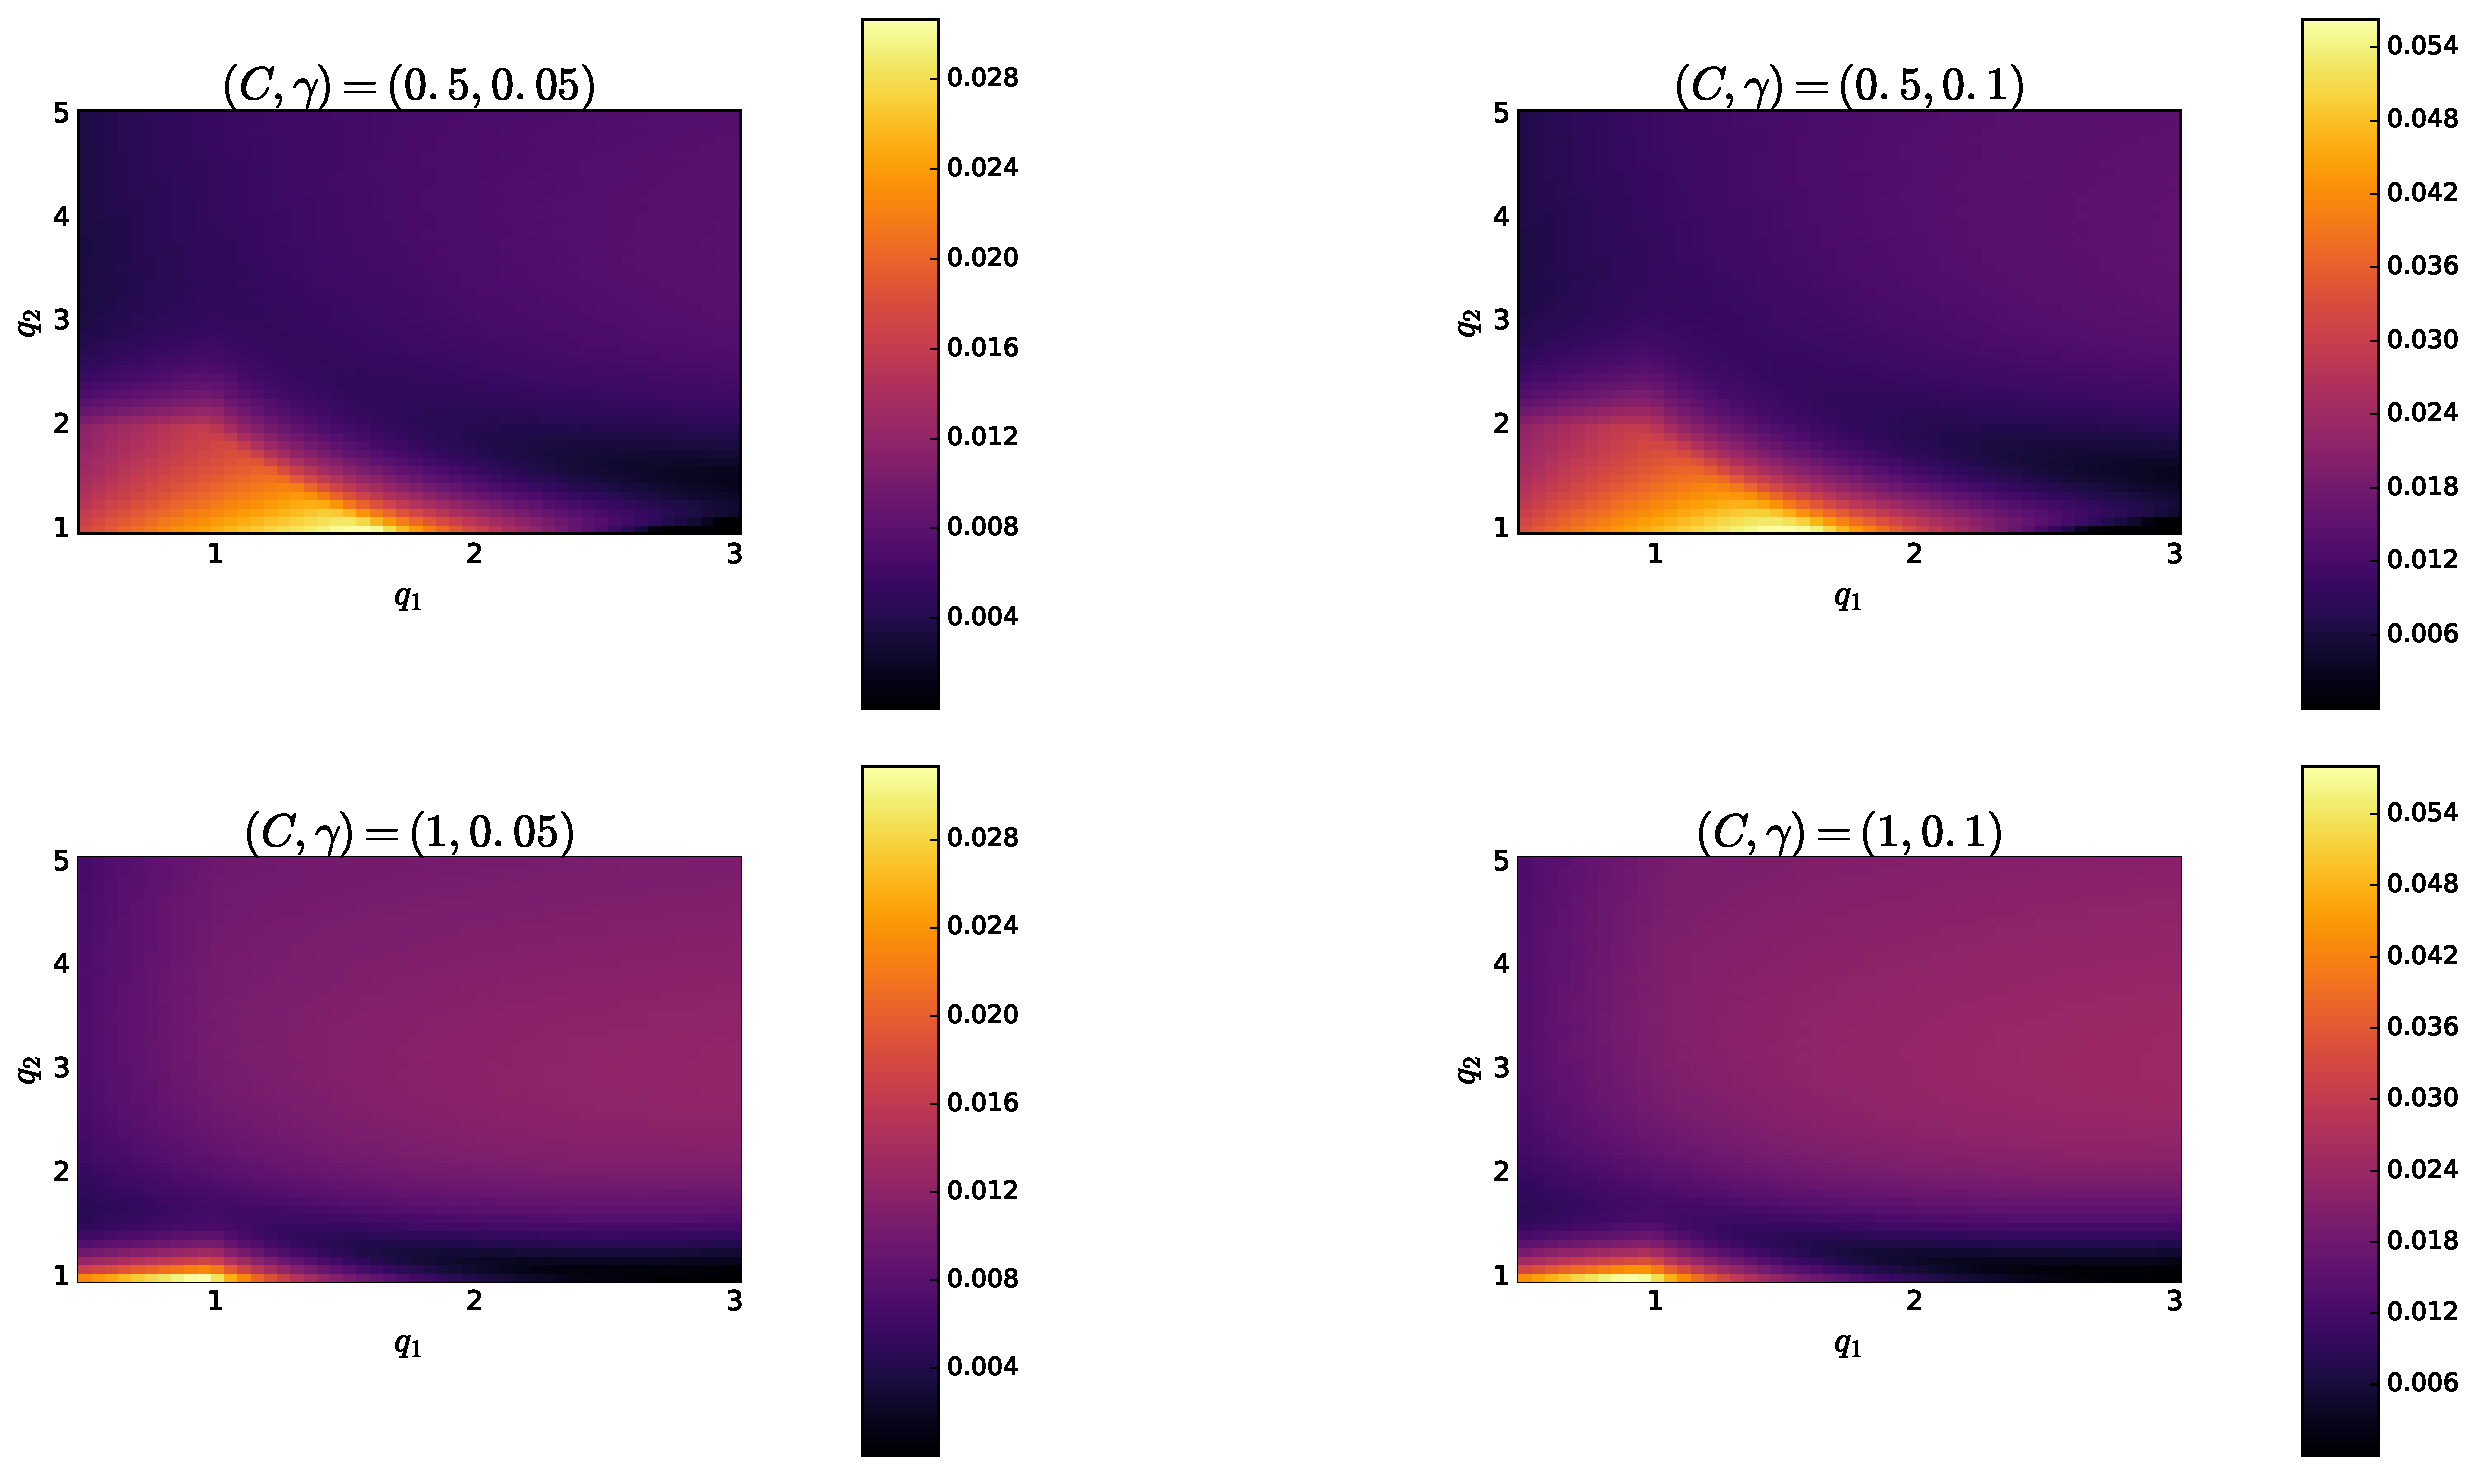
\includegraphics[width=0.96\textwidth]{./img/policy_diff_heatmaps}
  %\end{overpic}
  %\todo[inline]{Wrap PGF around raw heatmaps?}
  \caption{The $L^2$ difference $\|a^B(T-1,\cdot)-a^C(T-1,\cdot)\|_2$
    between the Bellman and CEC policy functions on $s\in[0,1]$.
    Each plot defines a combination of $(C,\gamma)$, whilst
    the axes vary the parameters $q_1,q_2$ of the demand function
    $q(a)=q_1e^{-q_2a}$.
    The difference is largest for small values of $q_1$ and $q_2$,
    which represent inelastic products with low absolute demand.
    The $L^2$ difference seems to scale uniformly over $(q_1,q_2)$, in the uncertainty
    parameter $\gamma$, with higher uncertainty increasing the
    difference.
    The white dot on the bottom, left plot corresponds to the
    parameters chosen for the experiments in this article.
  }\label{fig:policy_diff_heatmaps}
\end{figure}

The parameters chosen in this article's numerical experiments
are $C=1,\gamma=0.05,q_1=e^2/3\approx2.5,q_2=3$. This point lies
in the region where the $L^2$ difference is around $0.012$ --- see the
white dot in the
bottom, left subfigure in \Cref{fig:policy_diff_heatmaps}.
This difference is in the lower range of that seen for all the
combinations of parameters, so the conclusions made in the article
should be considered as relevant for a wider range of systems.

\biblio
\end{document}

%%% Local Variables:
%%% mode: latex
%%% TeX-master: t
%%% TeX-command-extra-options: "-shell-escape"
%%% End:
